% --- UNIVERSAL PREAMBLE BLOCK ---
\documentclass[11pt, a4paper]{article}
\usepackage[a4paper, top=2.5cm, bottom=2.5cm, left=2cm, right=2cm]{geometry}
\usepackage{fontspec}
\usepackage{graphicx}

\usepackage[english, provide=*]{babel}

\babelprovide[import, onchar=ids fonts]{english}

% Use XeLaTeX default font configuration for maximum portability

\usepackage{amsmath}

\title{\textbf{Conformational Free Energy Surface of Cyclohexane}}
\author{Ahmet Ekiz \\ MAT306 33975\\ Sabanci University}

\begin{document}

\maketitle

\section{Aim}
The primary objective of this study is to construct the conformational free energy surface of cyclohexane. To achieve this, the probability distributions of the ring's dihedral angles will be analyzed using trajectory data from 20 ns and 100 ns molecular dynamics (MD) simulations performed in NAMD at an elevated temperature of 1000 K. By applying the inverted Boltzmann equation, the observed probabilities will be converted into relative free energies. Ultimately, this approach will allow for the precise identification of the molecule's stable energy minima, transition barriers, and overall conformational energy distribution.

\section{Introduction}
\begin{figure}[htbp]
  \centering
  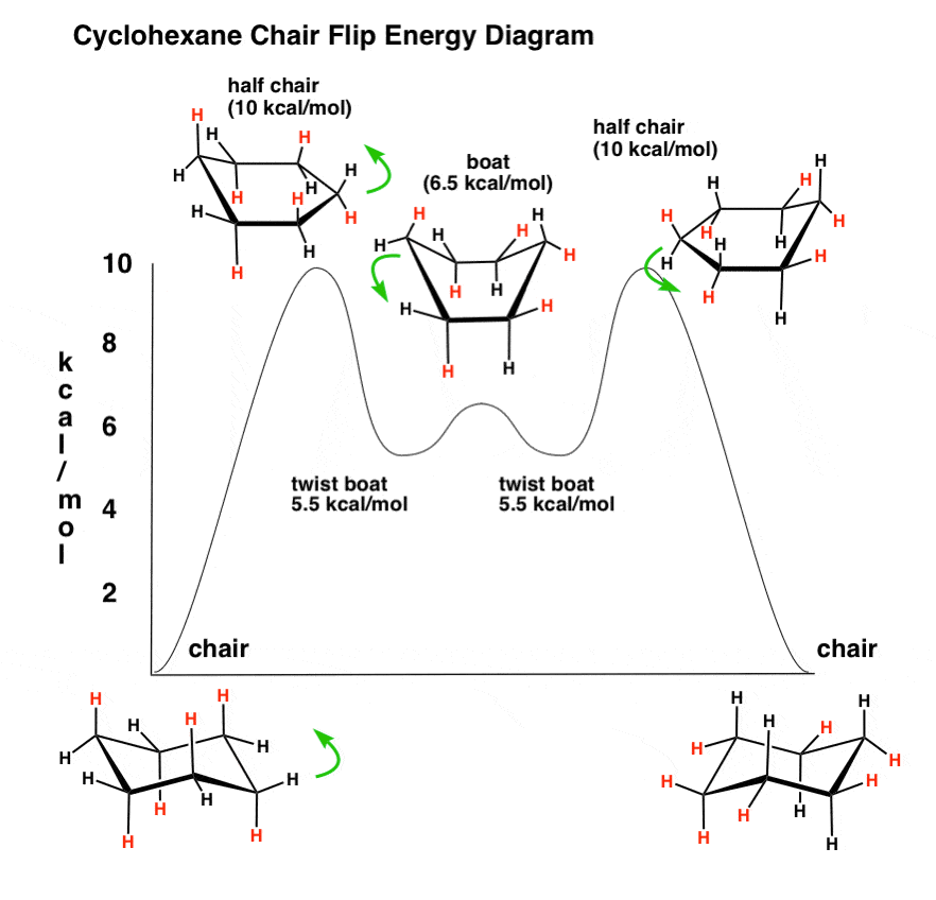
\includegraphics[width=0.6\textwidth]{Picture1.png}
  \caption{Cyclohexane Chair Flip Energy Diagram (Reference: masterorganicchemistry.com)}
  \label{fig:conformations}
\end{figure}

Unlike linear alkanes such as butane, which primarily exhibit simple \textit{trans} and \textit{gauche}$^\pm$ conformations, the cyclic structure of cyclohexane gives rise to a more complex conformational landscape. The molecule transitions between four primary states: the highly stable chair, the twist-boat, the boat, and the highly strained half-chair transition state. Mapping this free energy surface requires the molecule to broadly sample all possible geometries. The thermodynamic probability of overcoming energy barriers to reach these different states is governed by the Boltzmann factor:
\begin{equation}
P \propto e^{-\Delta E / RT}
\end{equation}

The energy barrier to undergo a "ring flip" (passing from a chair to a twist-boat via the half-chair) is experimentally known to be approximately 10.8 kcal/mol. At a standard room temperature of 300 K, the average available thermal energy ($RT$) is only $\approx 0.6$ kcal/mol. Because the barrier is 18 times larger than the available thermal energy, a room-temperature simulation would leave the molecule kinetically trapped in a single chair basin. By artificially elevating the simulation temperature to 1000 K, the thermal energy increases to $\approx 2.0$ kcal/mol. This significantly increases the probability of barrier crossing, allowing the system to thoroughly sample the rare transition states and alternative conformations over the 20 ns and 100 ns simulation timescales, yielding a mathematically complete view of the conformational surface.


\section{Methods}
Molecular dynamics (MD) simulations of a single cyclohexane ($C_6H_{12}$) molecule were performed using the NAMD software package. The system topology and atomic coordinates were provided, and the interactions were described using the CHARMM general parameter set (\texttt{par\_all35\_ethers-2.prm}), which explicitly includes the requisite C27 alkane parameters for carbon-carbon and carbon-hydrogen bonds. Two separate simulations were conducted for continuous durations of 20 ns and 100 ns, both utilizing a 1 fs integration timestep. 

To provide the system with sufficient kinetic energy to overcome the conformational ring-flip barriers, the simulation temperature was maintained at a constant 1000 K using a Langevin dynamics thermostat. The Langevin damping created a virtual thermal bath that stabilized the temperature and prevented extreme energy fluctuations. Notably, hydrogen atoms were intentionally excluded from this thermal coupling to prevent integration instabilities and unnatural high-frequency movements arising from their extremely low mass.

Trajectory analysis was performed using a custom Python script. The \texttt{MDAnalysis} library was utilized to extract two opposite dihedral angles of the carbon ring, specifically $\phi_1$ (C6-C1-C2-C3) and $\phi_2$ (C3-C4-C5-C6), at every saved frame. A 2D probability histogram was then generated from this data using the \texttt{NumPy} library. This probability distribution served as the foundation for the energy calculations, as it was mathematically inverted using the Boltzmann equation to map out the complete Free Energy Surface (FES).

\textbf{AI Disclosure:} Google Gemini 3.1 Pro was utilized during this assignment. Specifically, Gemini assisted in writing and debugging the NAMD configuration files, explaining the thermodynamic physics of Langevin damping, and developing the Python code used to extract the dihedral trajectory data and plot the surfaces.

\section{Results}
\begin{figure}[htbp]
  \centering
  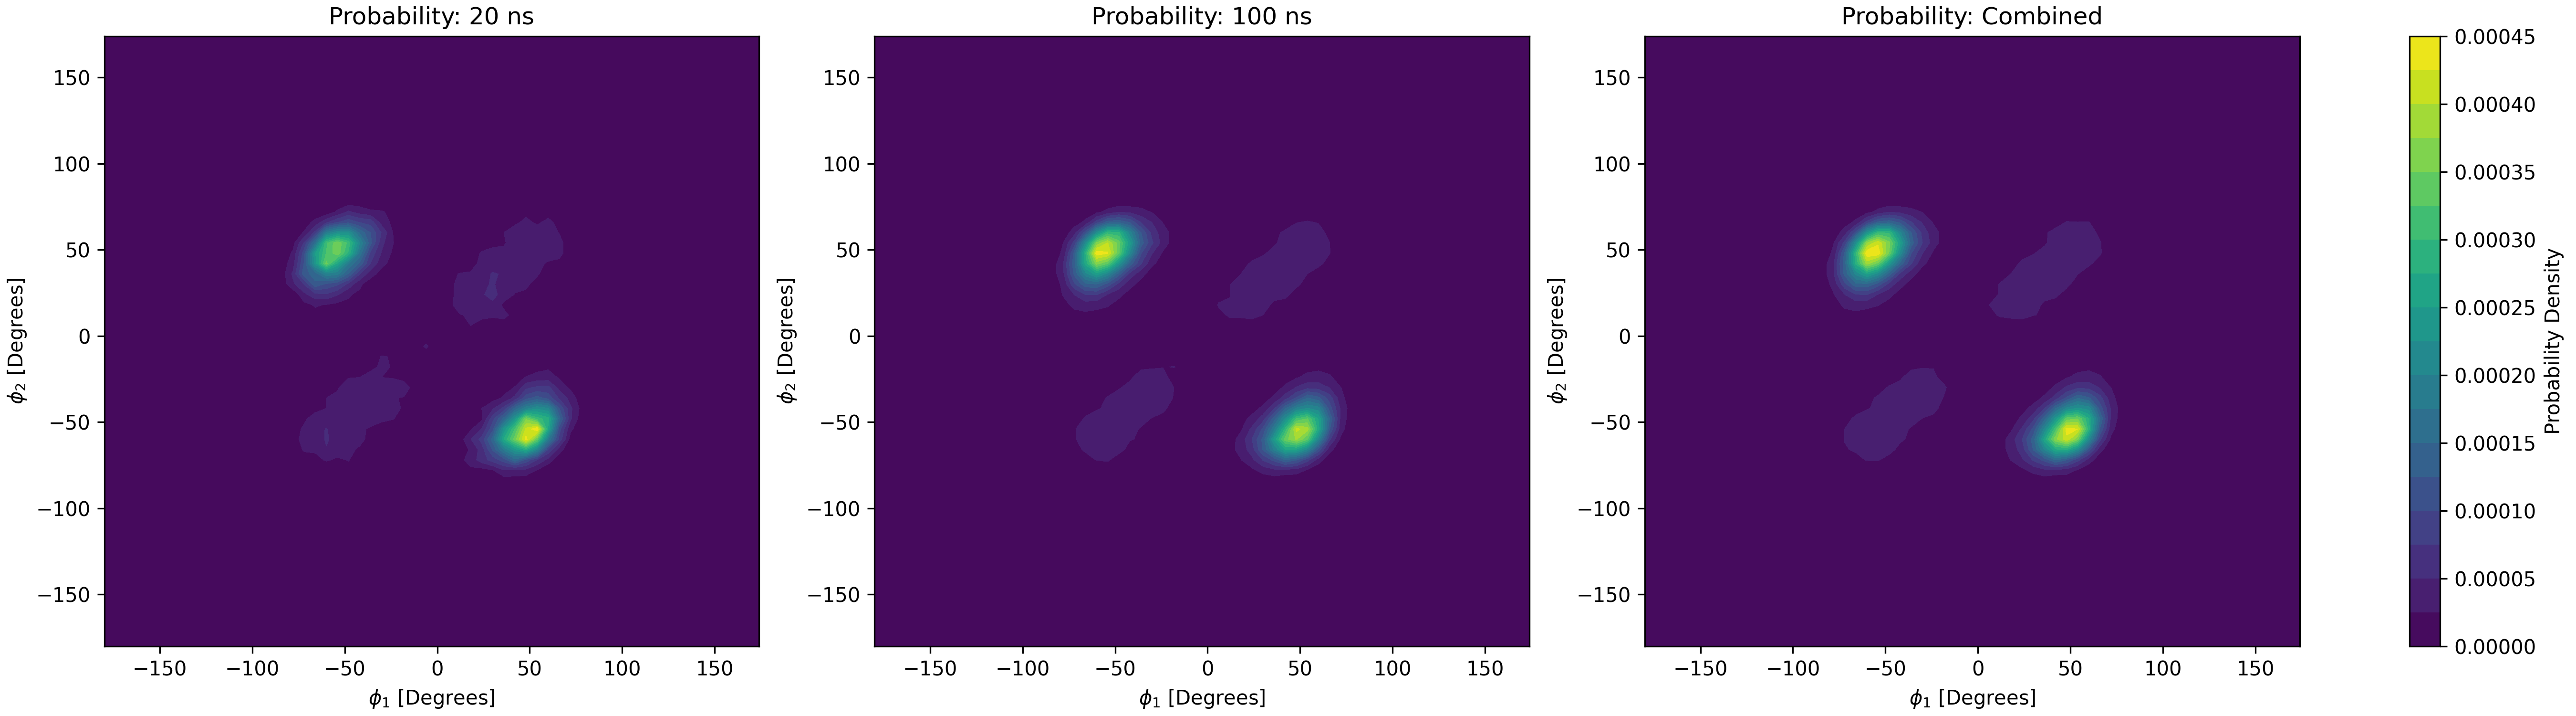
\includegraphics[width=\textwidth]{probability_surface_comparison_20ns_100ns_combined.png}
  \caption{Probability Surface comparison across different simulation lengths.}
  \label{fig:probability_comparison}
\end{figure}

\begin{figure}[htbp]
  \centering
  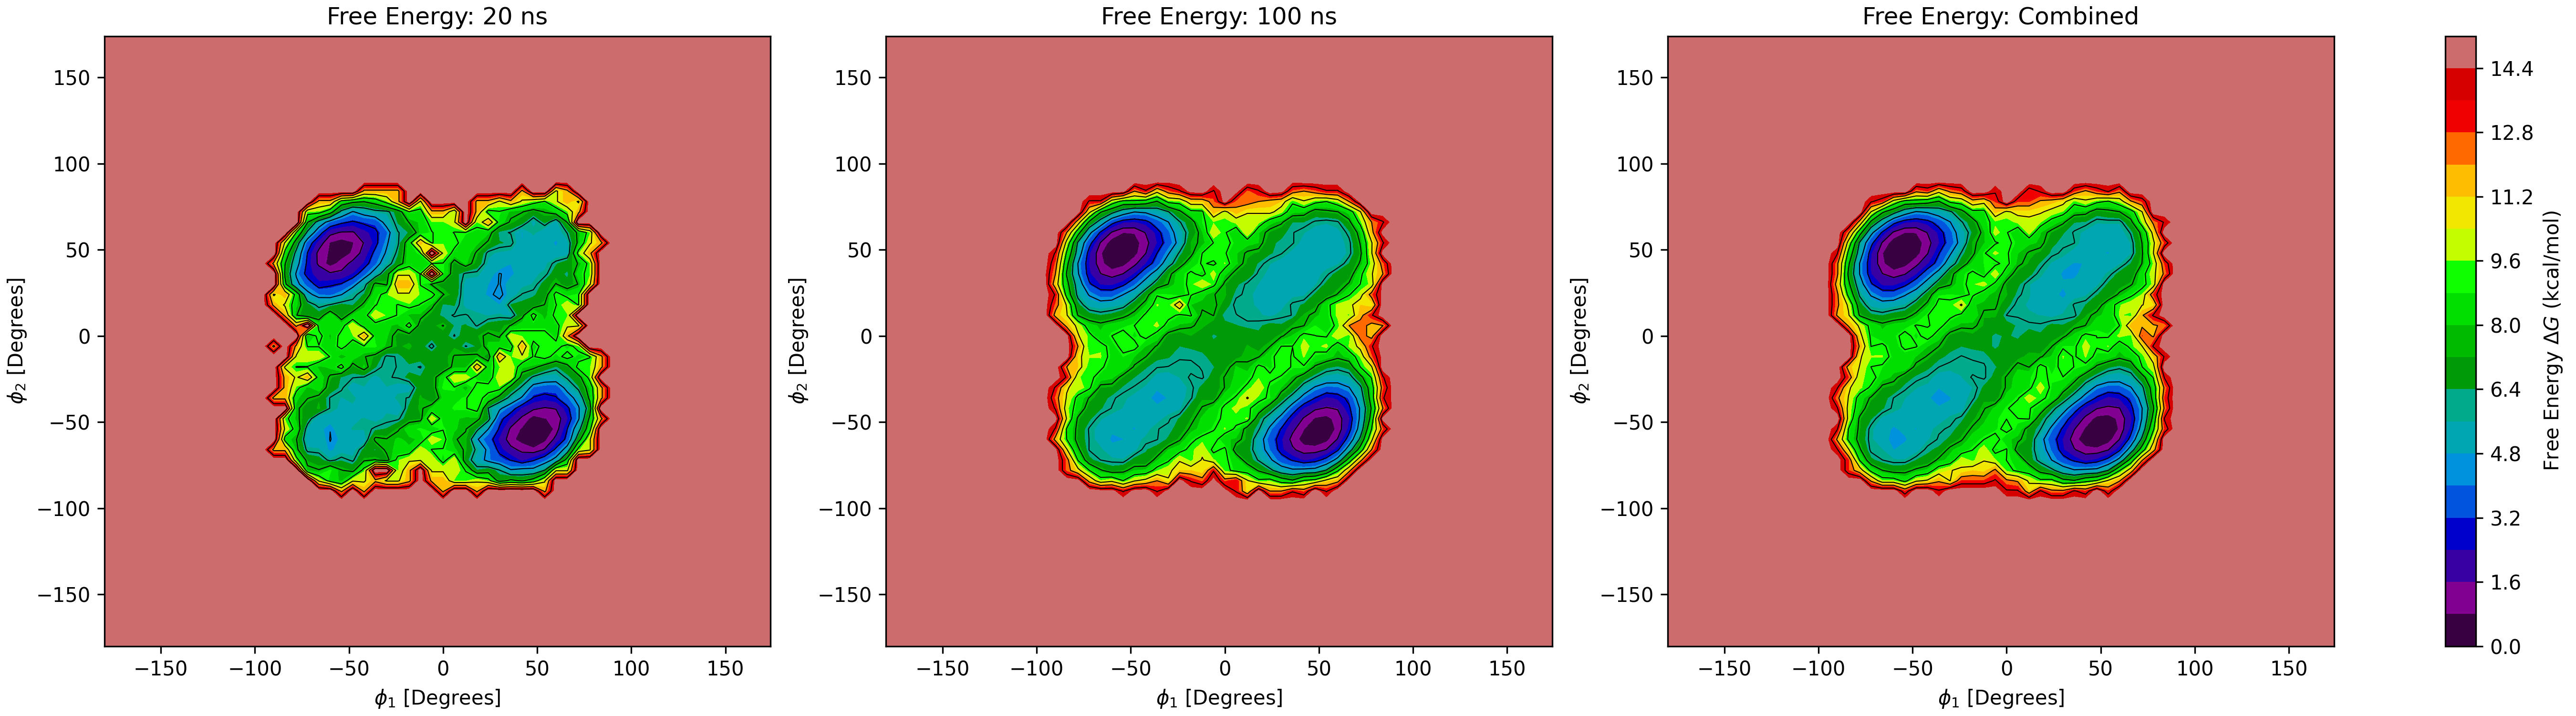
\includegraphics[width=\textwidth]{free_energy_surface_comparison_20ns_100ns_combined.png}
  \caption{Free Energy Surface ($\Delta G$) comparison across different simulation lengths at 1000 K.}
  \label{fig:energy_comparison}
\end{figure}

The most stable form of cyclohexane, the chair conformation, is set as 0 kcal/mol to serve as our thermodynamic reference point. The computed Free Energy Surface (FES) and Probability Surface are both highly symmetric, reflecting the underlying symmetry of the cyclohexane ring. The global minima, corresponding to the chair conformations, are located at ($\phi_1 \approx -50^\circ, \phi_2 \approx 50^\circ$) and ($\phi_1 \approx 50^\circ, \phi_2 \approx -50^\circ$). Additionally, local minima representing the twist-boat conformations are found at ($\phi_1 \approx 50^\circ, \phi_2 \approx 50^\circ$) and ($\phi_1 \approx -50^\circ, \phi_2 \approx -50^\circ$). These twist-boat states possess a relative free energy of approximately 5.5 kcal/mol, which aligns perfectly with the observed contour range of 4.8--6.4 kcal/mol.

By comparing the 20 ns, 100 ns, and combined datasets (Figures \ref{fig:probability_comparison} and \ref{fig:energy_comparison}), the impact of extended simulation times on conformational sampling becomes evident. While the initial 20 ns simulation successfully identifies the deep local and global minima, the high-energy transition pathways remain somewhat sparsely sampled and topologically noisy. 

Extending the simulation to 100 ns and combining the datasets significantly smooths the conformational landscape. With the combined dataset, the transition states are distinctly resolved. The pure boat conformation, acting as a saddle point at ($\phi_1 \approx 0^\circ, \phi_2 \approx 0^\circ$), becomes clearly defined at approximately 7.5 kcal/mol. Furthermore, the highest energy ridges representing the half-chair transition state form continuous, well-defined barriers peaking at roughly 10.5 kcal/mol. This demonstrates that the extended timeframe allows the system to cross the massive energy barriers more frequently, yielding a statistically complete picture of the rare transition states rather than just the stable valleys.

\begin{table}[htbp]
  \centering
  \begin{tabular}{llc}
    \hline
    \textbf{Conformational State} & \textbf{Topological Feature} & \textbf{Relative Free Energy ($\Delta G$)} \\
    \hline
    Chair & Global Minimum & 0.0 kcal/mol \\
    Twist-Boat & Local Minimum & $\sim 5.5$ kcal/mol \\
    Boat & Saddle Point / Transition & $\sim 7.5$ kcal/mol \\
    Half-Chair & Primary Energy Barrier & $\sim 10.5$ kcal/mol \\
    \hline
  \end{tabular}
  \caption{Summary of calculated relative free energies for primary cyclohexane conformations.}
  \label{tab:energies}
\end{table}

\section{Conclusions}
By elevating the simulation temperature from 300 K to 1000 K, the system was provided with sufficient thermal energy to overcome the high-energy half-chair barriers. This approach successfully prevented kinetic trapping, allowing the molecule to thoroughly explore its conformational phase space. Consequently, the combination of extended simulation time (100 ns) and elevated temperature yielded a highly resolved and statistically complete free energy surface.

However, this high-temperature methodology introduces physically unrealistic artifacts. Simulating at 1000 K implicitly relies on classical harmonic force fields to maintain structural integrity under extreme thermal stress. In reality, at such elevated temperatures, standard bonds are not strictly unbreakable, and the effects of quantum dynamics and potential bond dissociation become significant. To obtain a chemically accurate free energy surface at a biologically relevant 300 K without artificial heating, advanced enhanced sampling techniques (such as Umbrella Sampling or Metadynamics) should be utilized. Furthermore, explicitly studying high-energy bond vibrations or breaking would require reactive force fields (e.g., ReaxFF in LAMMPS) or \textit{ab initio} molecular dynamics (AIMD).

\end{document}